\documentclass{beamer}
\usepackage[english]{babel}
\usepackage[T1]{fontenc}

% other packages
\usepackage{latexsym,amsmath,xcolor,multicol,booktabs,calligra}
\usepackage{graphicx,pstricks,listings,stackengine}

\author{\href{}{Vidipt Vashist \\ (MA22M025)}}
\institute{\href{}{Indian Institute of Technology Madras \\
Department of Mathematics\\
MA5990 M.Tech Project}}
\title{Chatbot based on Retrieval Augmented Generation (RAG)}
\date{\today}
\usepackage{Amr_Beamer}

% defs
\def\cmd#1{\texttt{\color{red}\footnotesize $\backslash$#1}}
\def\env#1{\texttt{\color{blue}\footnotesize #1}}
\definecolor{deepblue}{rgb}{0,0,0.5}
\definecolor{deepred}{rgb}{0.6,0,0}
\definecolor{deepgreen}{rgb}{0,0.5,0}
\definecolor{halfgray}{gray}{0.55}

\lstset{
    basicstyle=\ttfamily\small,
    keywordstyle=\bfseries\color{deepblue},
    emphstyle=\ttfamily\color{deepred},   % Custom highlighting style
    stringstyle=\color{deepgreen},
    numbers=left,
    numberstyle=\small\color{halfgray},
    rulesepcolor=\color{red!20!green!20!blue!20},
    frame=shadowbox,
}


\begin{document}


\begin{frame}
    \titlepage
    \begin{figure}
    
\includegraphics[width=0.07\textwidth]{pic/logored.png}
        
    \end{figure}
\end{frame}

\begin{frame}
    \tableofcontents[sectionstyle=show,subsectionstyle=show/shaded/hide,subsubsectionstyle=show/shaded/hide]
\end{frame}


\section{INTRODUCTION}

\begin{frame}{INTRODUCTION}
\begin{itemize}
    

\item RAG is is a \textbf{groundbreaking paradigm} in natural language processing that 
combines the strengths of retrieval-based and generation-based approaches. 

\item It's a \textbf{ AI framework} for retrieving facts from an external knowledge base to ground large language models (LLMs) on the most accurate, up-to-date information and to give users insight into LLMs' generative process.
.

\item This innovative \textbf{framework 
combines the best aspects of different methodologies to achieve impressive results} in a wide range of NLP 
tasks, including question answering and text summarization, among others.
\end{itemize}




\end{frame}


\begin{frame}{TECHNICAL OVERVIEW OF RAG}
    \begin{figure}
    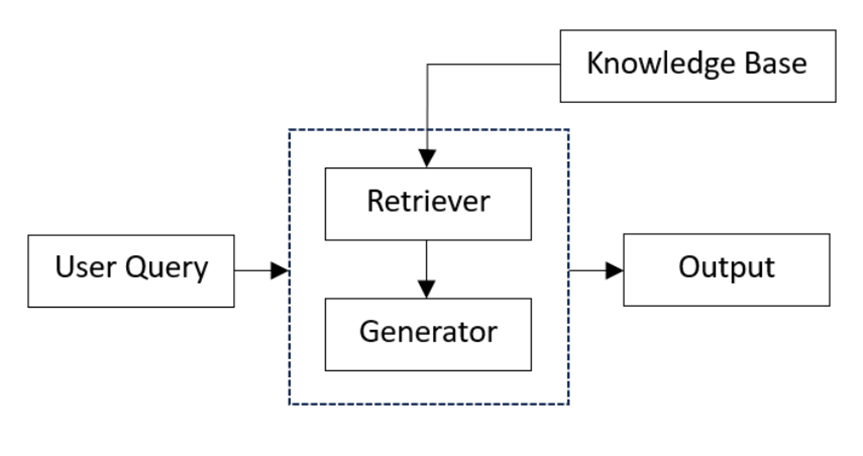
\includegraphics[width=0.7\textwidth]{F1.png}
    \end{figure}

    \begin{center}
            \textbf{Core Idea:} Retriever + Generation 

    \end{center}

\end{frame}



\begin{frame}{TECHNIQUES LANDSCAPE}
    \begin{figure}
    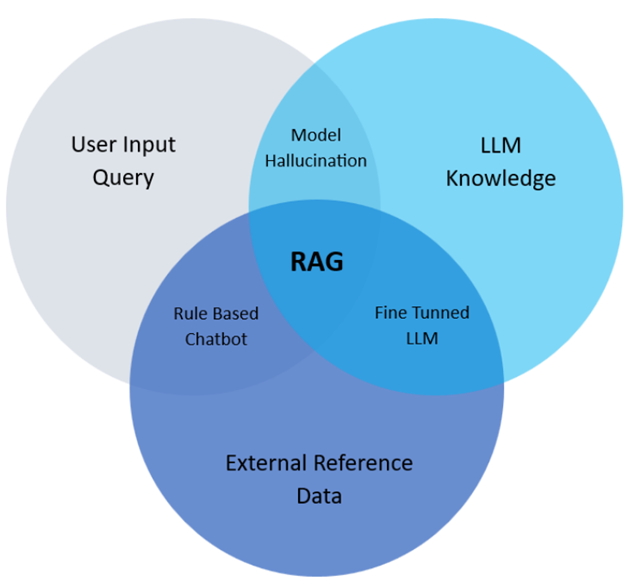
\includegraphics[width=0.7\textwidth]{F2.png}
        
    \end{figure}
    
\end{frame}

\begin{frame}{WHY RAG ?}
\begin{itemize}
    \item  \textbf{Reduced Hallucinations:} models exhibit fewer hallucinations and 
higher response accuracy.
\item  \textbf{Enhanced LLM Memory:}  the information capacity limitation of traditional 
Language Models (LLMs). Traditional LLMs have a limited memory. 
RAG introduces memory by tapping into external knowledge sources.

\item \textbf{Updatable Memory:} is its ability to accommodate real-time updates 
and fresh sources without extensive model retraining. 
information
\item \textbf{Improved Contextualization:}  enhances the contextual understanding of LLMs by retrieving 
and integrating relevant contextual documents.
\end{itemize}


    
\end{frame}

\section{PROBLEM STATEMENT}

\begin{frame}{PROBLEM STATEMENT}

The main goal of this project is to achieve two things:   \\

 \begin{itemize}
     \item  firstly, to create a reliable and open-source system 
that can efficiently extract information from private PDF files: \textbf{Internal Document RAG System}
\item and secondly, to develop a user-friendly 
web application that utilizes web scraping techniques to gather relevant data from online sources: \textbf{Web Search RAG System}

 \end{itemize}
 
\end{frame}


\begin{frame}{INTERNAL DOCUMENT RAG SYSTEM}

\textbf{Current Challenges}
    \begin{itemize}
        \item Extracting information from private PDF files can pose significant challenges for organizations,
        leading to complexity and inefficiency in their data extraction processes.
        \item This challenge impedes their capacity to effectively utilize internal knowledge,
        \item Resulting in missed chances for improved customer interactions and a competitive advantage in the market
    \end{itemize}   
\begin{block}{Solution}
to create a reliable and open-source system that can efficiently extract information from private PDF files \end{block}

\end{frame}

\begin{frame}{WEB SEARCH RAG SYSTEM}

\textbf{Current Challenges}
 
    \begin{itemize}
        \item Navigating the vast expanse of the internet can be quite the challenge when it comes to finding relevant and accurate information in a timely manner.
        \item Many users struggle to refine their search queries for more accurate results. 
        \item In addition, current search engines often fail to offer a complete context to improve the user's comprehension of the retrieved data.
    \end{itemize}   
\begin{block}{Solution}
to develop a user-friendly web application that utilizes web scraping techniques to gather relevant data from online sources.
\end{block}

\end{frame}







\section{METHODOLOGY}

\begin{frame}{HIGH LEVEL TECHNICAL FLOW}
    \begin{figure}
    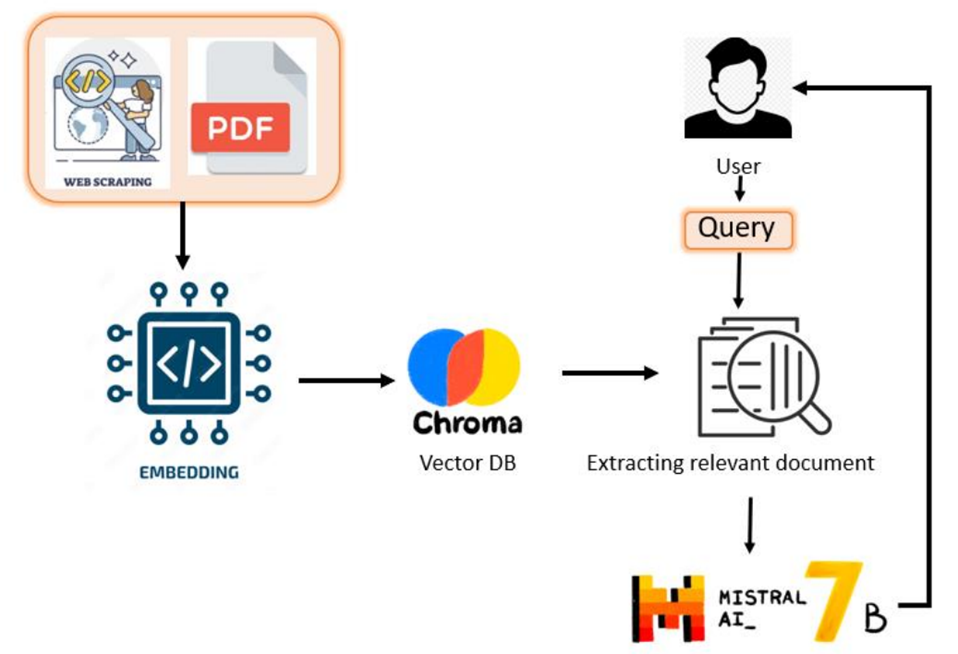
\includegraphics[width=0.7\textwidth]{F3.png}
        
    \end{figure}
\begin{center}
    for showcasing technology frame work used for project.
\end{center}
     

\end{frame}




\begin{frame}{CUSTOM ARCHITECTURE}
\begin{center}
        \begin{figure}
    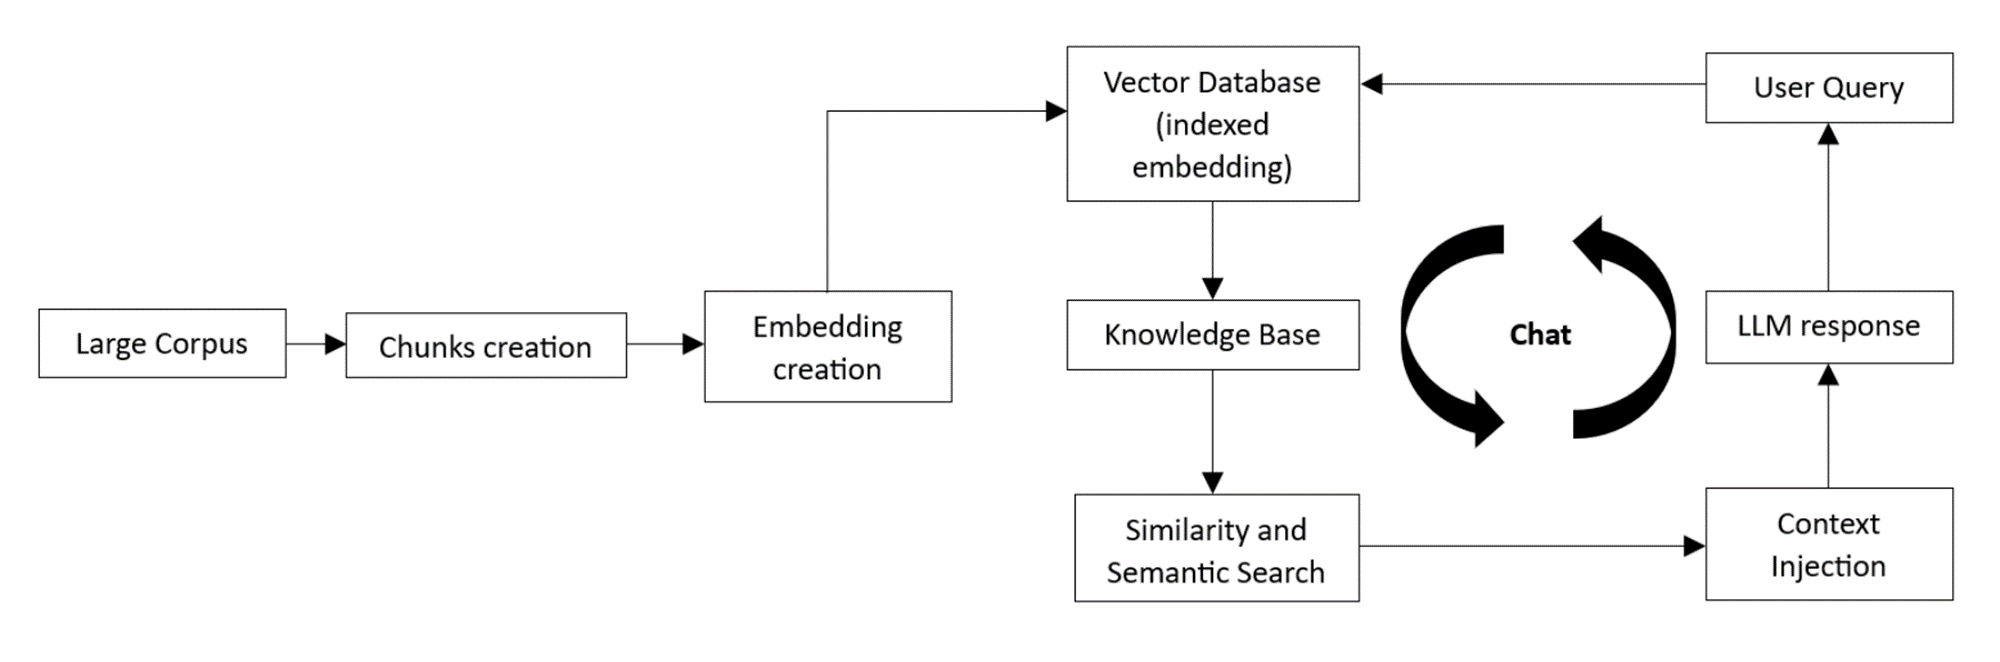
\includegraphics[width=1\textwidth]{F4.png}
        
    \end{figure}
\end{center}

    \begin{center}
        Custom Architecture for RAG system

    \end{center} 

\end{frame}

\begin{frame}{FRAMEWORK + HARDWARE RESOURCE}

\textbf{FRAMEWORK}
\begin{itemize}
    

\item Document Ingestion: Llama Index
\item Creating Embedding: all-MiniLM-L6-v2 Architecture
\item Vector Database: Chroma DB
\item Generator: Mistral-7B-Instruct-v0.2
\item Support framework: Langchain
\end{itemize}
\\ \\


\textbf{HARDWARE RESOURCE}
\begin{itemize}
    

\item GPU: P100 (16 GB)
\item CPU: 29 GB
\item DISK: 75 GB
\end{itemize}
\end{frame}







\section{LIVE DEMO}
\begin{frame}{}
    \centering
    \Huge % Set the font size to be large
    LIVE DEMO FOR PROJECT % Your live demo content goes here

    \small
\begin{enumerate}
    \item Internal Document Search RAG System
    \item Web Search RAG System
\end{enumerate}
\end{frame}




\section{FUTURE SCOPE}

\begin{frame}{Future Scope}

As technology continues to evolve and new challenges emerge for future work, ranging from the exploration of new large language models (LLMs) to the advancement of RAG architectures: 
\begin{itemize}


    \item Integration of Multimodal Information
    \item Fine-Tuning Techniques and Optimization
    \item Addressing Privacy and Security Concerns
\end{itemize}
\end{frame}

\begin{frame}{}
    \centering
    \Huge % Set the font size to be large
    THANK YOU % Your live demo content goes here


\end{frame}
\end{document}
